\section{Stima della corrente di attivazione}

\begin{wrapfigure}[14]{r}[0pt]{100mm}
	\centering
    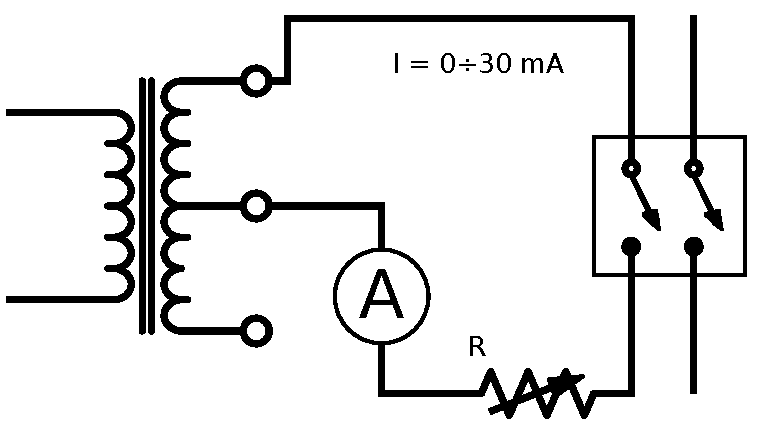
\includegraphics[width=0.40\textwidth]{amper.pdf}
    \caption{Schema del circuito utilizzato per la misura differenziale di corrente.}
    \label{fig:amper}
\end{wrapfigure}

L'interruttore differenziale sfrutta l'induzione magnetica per rilevare perdite di corrente e intervenire aprendo il circuito. Esso ha al suo interno due bobine avvolte in modo che, quando il circuito funziona correttamente, ovvero la corrente in uscita eguaglia la corrente in entrata, i campi magnetici generati dalle bobine si annullano a vicenda. Quando invece si ha una perdita di corrente (ad esempio a terra), i campi magnetici generati sono diversi e si ha dunque un effetto di induzione elettromagnetica su una terza bobina che, attivando un meccanismo, apre il circuito.

Come mostrato in Fig. \ref{fig:amper}, abbiamo montato il circuito facendo passare un solo cavo nell'interruttore differenziale. Così facendo, abbiamo simulato il caso in cui la perdita di corrente è del 100\% a terra. Misurando poi, attraverso il multimetro, per quale valore di corrente l'interruttore scattava e ripetendo le misure varie volte, abbiamo stimato un valore di corrente di attivazione. 

Avendo alimentato il circuito con una tensione alternata a $7.5V_{rms}$, abbiamo utilizzato una decade di resistenze per poter ottenere diversi valori di corrente nel circuito. Sono stati eseguiti 15 campionamenti, con valor medio di corrente efficace $I_{eff} =  (26.5\pm0.3)\si{\milli\ampere}$. Abbiamo osservato che il valore di corrente di attivazione si aveva per un valore di resistenza di circa $300\si{\ohm}$. 


\section{Stima del tempo di intervento}

\begin{wrapfigure}[14]{r}[0pt]{100mm}
	\centering
    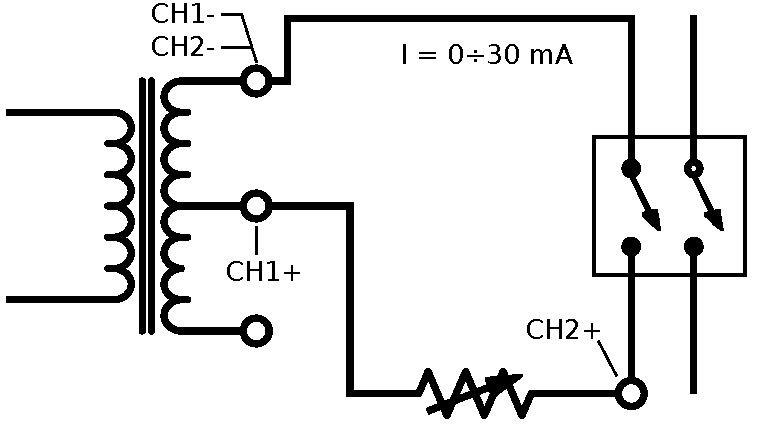
\includegraphics[width=0.40\textwidth]{time.pdf}
    \caption{Schema del circuito utilizzato per la stima del tempo di intervento.}
    \label{fig:time}
\end{wrapfigure}

Per stimare il tempo di intervento dell'interruttore abbiamo utilizzato l'oscilloscopio in modalità acquisizione singola. In questa modalità lo strumento inizia a prendere dati solo nel momento in cui rileva un segnale, facendone un'istantanea sullo schermo. Risulta così possibile osservare un fenomeno isolato e non periodico bloccandone l'immagine e analizzandola successivamente.

Come mostrato in Fig. \ref{fig:time}, sono stati collegati i canali dell'oscilloscopio in modo da avere sullo schermo sempre il segnale ai capi del generatore di tensione e quello ai capi dell'interruttore differenziale. Così facendo, fino a quando l'interruttore differenziale rimane chiuso, la ddp ai suoi capi sarà nulla mentre dopo l'apertura osserveremo un andamento identico a quello in input.

Per stimare il tempo di intervento abbiamo spento il generatore di tensione, impostata una resistenza bassa (inferiore a quella di soglia stimata nella sezione precedente) e chiuso l'interruttore. Dopo aver impostato l'oscilloscopio in acquisizione singola, abbiamo acceso il generatore di tensione. Sullo schermo abbiamo ottenuto una figura come quella riportata in Fig. \ref{fig:graph}.

\begin{figure}[h]
	\centering
    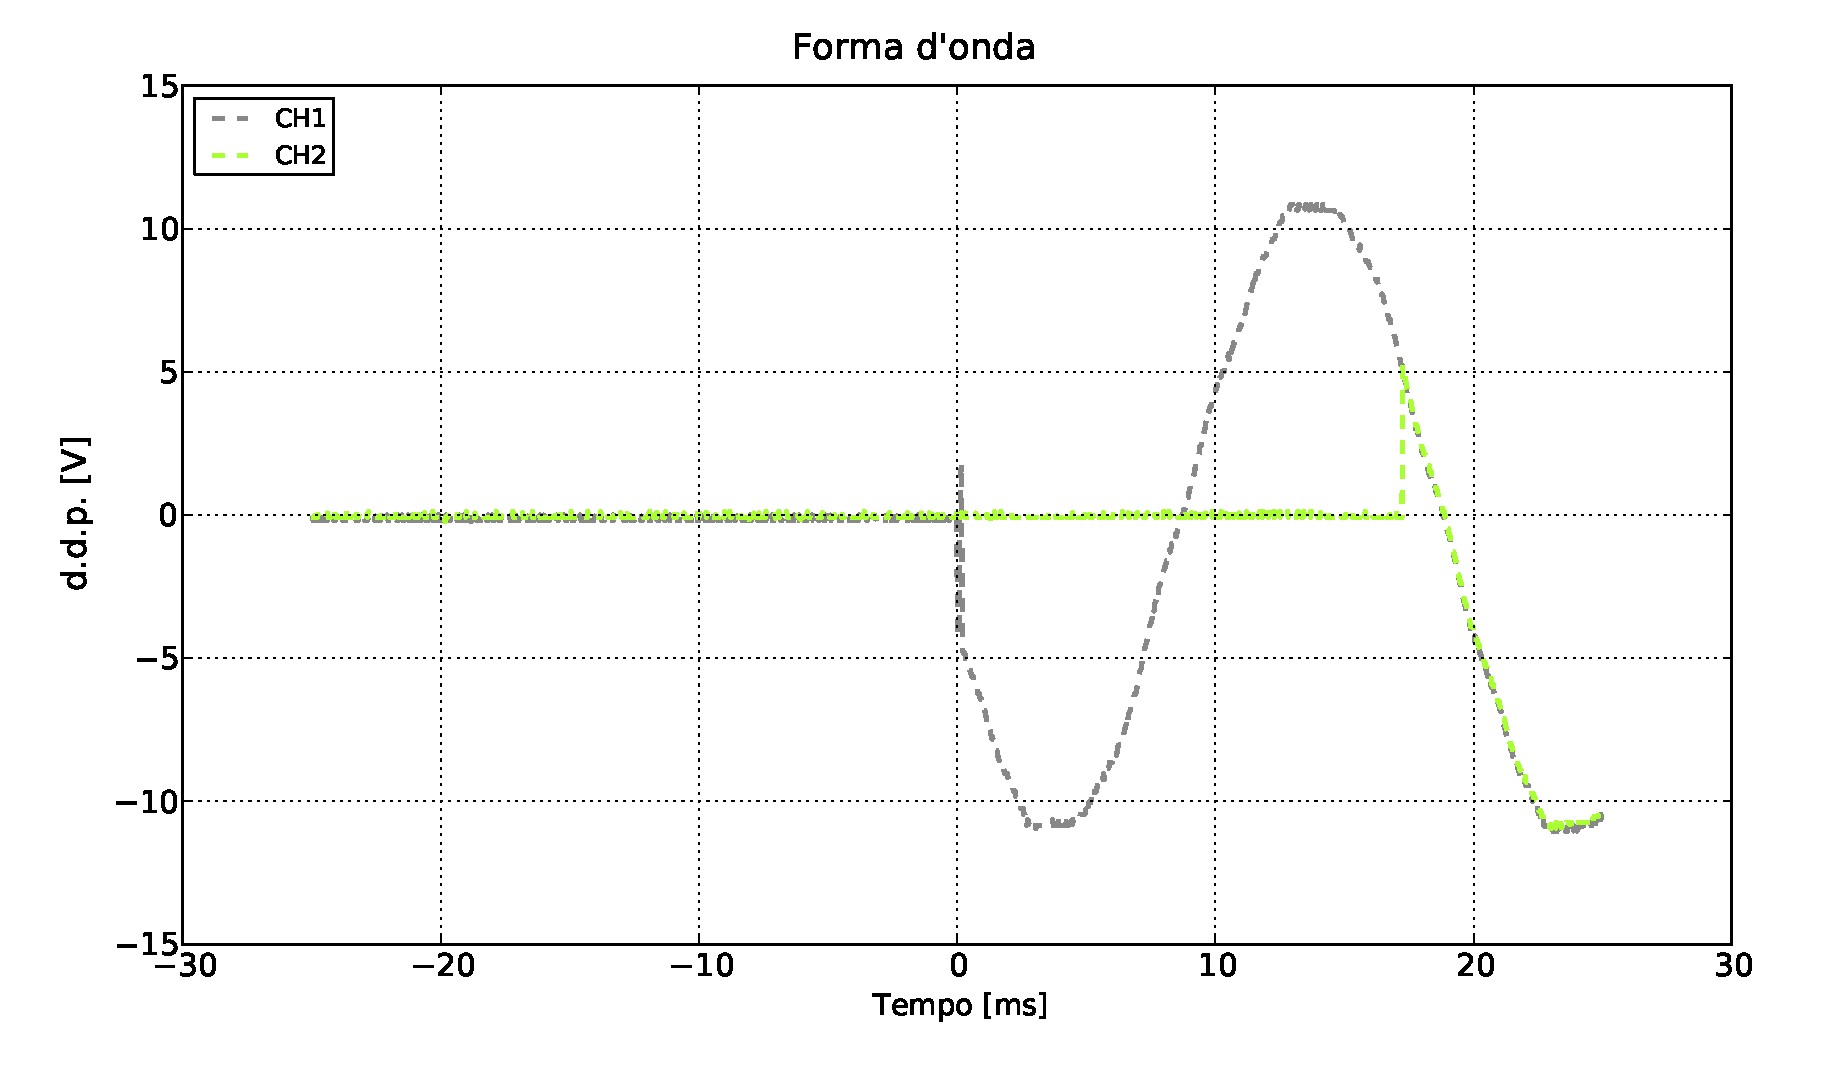
\includegraphics[height=3in]{graph.pdf}
    \caption{Grafico dei segnali su i due canali dell'oscilloscopio per la resistenza da $\SI{249.97}{\ohm}$.}
    \label{fig:graph}
\end{figure}


Utilizzando i puntatori sullo schermo, abbiamo stimato il valore di $t_{att}$ che intercorreva tra il momento di accensione del generatore (quando compare il segnale sullo schermo riferito al CH1) e il momento in cui lo stesso segnale appariva su CH2. Abbiamo notato che tale intervallo di tempo era fortemente variabile (anche $8\si{\milli\second}$ per lo stesso valore di resistenza). Inoltre, provando con diversi valori di resistenza $R$ si è notato che mediamente il tempo di intervento aumentava. Ricordiamo che il valore di $V_0 \, = \, \SI{7.5}{\volt}_{rms}$. Sono stati eseguiti 5 campionamenti per ciascuna resistenza. Riportiamo in tabella i valori medi di tempo di intervento.

\begin{table}[h]
\centering
\caption{Media dei tempi di intervento dell'interruttore differenziale per diversi valori di $R$.}
{\renewcommand{\arraystretch}{1.6}%
\begin{tabular}{c|c|c|c|c}
 & $R=50 \si{\ohm}$ & $R=100 \si{\ohm}$ & $R=200 \si{\ohm}$ & $R=250 \si{\ohm}$ \\      \hline
$t_{att}$ [$\si{\milli\second}$] & $(13 \pm 2)$ & $(14 \pm 2)$ & $(18 \pm 7)$ & ($20 \pm 4$) \\\end{tabular}}
\end{table}


Il valore massimo di tempo campionato risulta essere $29.4\si{\milli\second}$ misurato con una resistenza di $R=250 \si{\ohm}$ mentre quello minimo $11.2\si{\milli\second}$ ottenuto nel caso di resistenza $R=50 \si{\ohm}$.

Abbiamo casualmente notato che, sebbene i tempi di attivazione a parità di resistenza fossero diversi, il tempo tra l'ultimo passaggio del segnale sull'asse delle $x$ e l'apertura dell'interruttore rimaneva costante (Fig. \ref{fig:graph}). Abbiamo dunque ipotizzato l'esistenza di un tempo di attivazione ``meccanico'', ovvero dal momento in cui l'interruttore è attraversato da una differenza di corrente critica e inizia il processo meccanico di apertura del circuito fino al completamento dello stesso, e che esso fosse una costante (che chiameremo $\tau$).  Riportiamo i tempi tra l'ultimo passaggio del segnale sull'asse $x$ e l'apertura del circuito nella seguente tabella. 

\begin{table}[h]
\centering
\parbox{14 cm}{\caption{Media dei tempi tra ultimo passaggio della sinusoide sull'asse dei tempi e intervento dell'interruttore per diversi valori di $R$.}}
{\renewcommand{\arraystretch}{1.6}%
\begin{tabular}{c|c|c|c|c}
 & $R=50 \si{\ohm}$ & $R=100 \si{\ohm}$ & $R=200 \si{\ohm}$ & $R=250 \si{\ohm}$ \\      \hline
$\Delta t$ [$\si{\milli\second}$] & $(5.4 \pm 0.1)$ & $(6.2 \pm 0.1)$ & $(7.7 \pm 0.1)$ & ($8.5 \pm 0.1$) \\
\end{tabular}}
\end{table}

Come vediamo, i valori variano al variare della resistenza. Ciò è coerente con il fatto che a parità di tensione, con resistenze più alte scorre meno corrente. Inoltre, l'interruttore differenziale sfrutta le variazioni di corrente, pertanto esso sarà sensibile alla derivata della corrente.
% provo a riscrivere questa parte come la vedo io % la tua l'ho copiata in puffo.txt

\noindent Ricordiamo che $V_0 \, = \, V_{eff} \sqrt{2}$ e $I_0 \, = \, I_{eff} \sqrt{2}$, assumiamo una forma della corrente\footnote{In realtà $I(t)=\frac{V_0}{R}cos(\omega t + \varphi)$, non è tuttavia restrittivo ai fini della teoria supporre $\varphi$ uguale a zero poiché il valore di $\tau$ è indipendente dalla fase $\varphi$} del tipo:
\begin{equation}
I(t)=\frac{V_0}{R}cos(\omega t)
\label{eq:corrente}
\end{equation}

Risulta banale calcolare la sua derivata temporale:

\begin{equation}
\frac{dI(t)}{dt}=-\frac{V_0 \omega}{R}sin(\omega t)
\label{eq:derivata}
\end{equation}

\noindent La variazione di corrente farà quindi scattare l'interruttore quando il suo valore sarà, in modulo, maggiore o uguale ad una determinata costante ($K$). Il caso limite si ottiene con la corrente di attivazione, ovvero con $R \simeq \SI{300}{\ohm}$: in tale caso l'interruttore si aprirà solo quando la derivata della corrente sarà massima, cioè per $sin(\omega t) = 1$.

\begin{equation}
\frac{V_0 \omega}{R}|sin(\omega t)| \, \geq \, K	\quad \longrightarrow  \quad	
\left\vert \frac{dI(t)}{dt} \right\vert_{max} = \frac{V_0 \omega}{R} = K
\label{eq:max}
\end{equation}

\noindent Grazie al valore di $I_{eff}$ ottenuto nella parte precendente dell'esperienza possiamo ricavare $K$:

\begin{equation}
K = \frac{V_0 \omega}{R} = I_0 \,\omega = \sqrt{2}\,I_{eff} \,\omega  = (11.8 \pm 0.1)\, \si{\ampere\per\second}
\label{eq:K}
\end{equation}

\noindent Dalle diverse serie di dati invece, grazie a $K$, possiamo ricavare invertendo (\ref{eq:max}) il tempo $t^*$ a cui la derivata della corrente diventa uguale al valore necessario per far scattare l'interruttore. La relazione usata è la seguente:

\begin{equation}
t^* \, = \, \frac{1}{\omega}arcsin\left(\frac{K R}{V_0 \omega}\right)
\label{eq:t_star}
\end{equation}

Non rimane che stimare il tempo di attivazione \emph{meccanico} $\tau$ grazie alla seguente relazione,
\begin{wrapfigure}[24]{r}[0pt]{110mm}
	\centering
    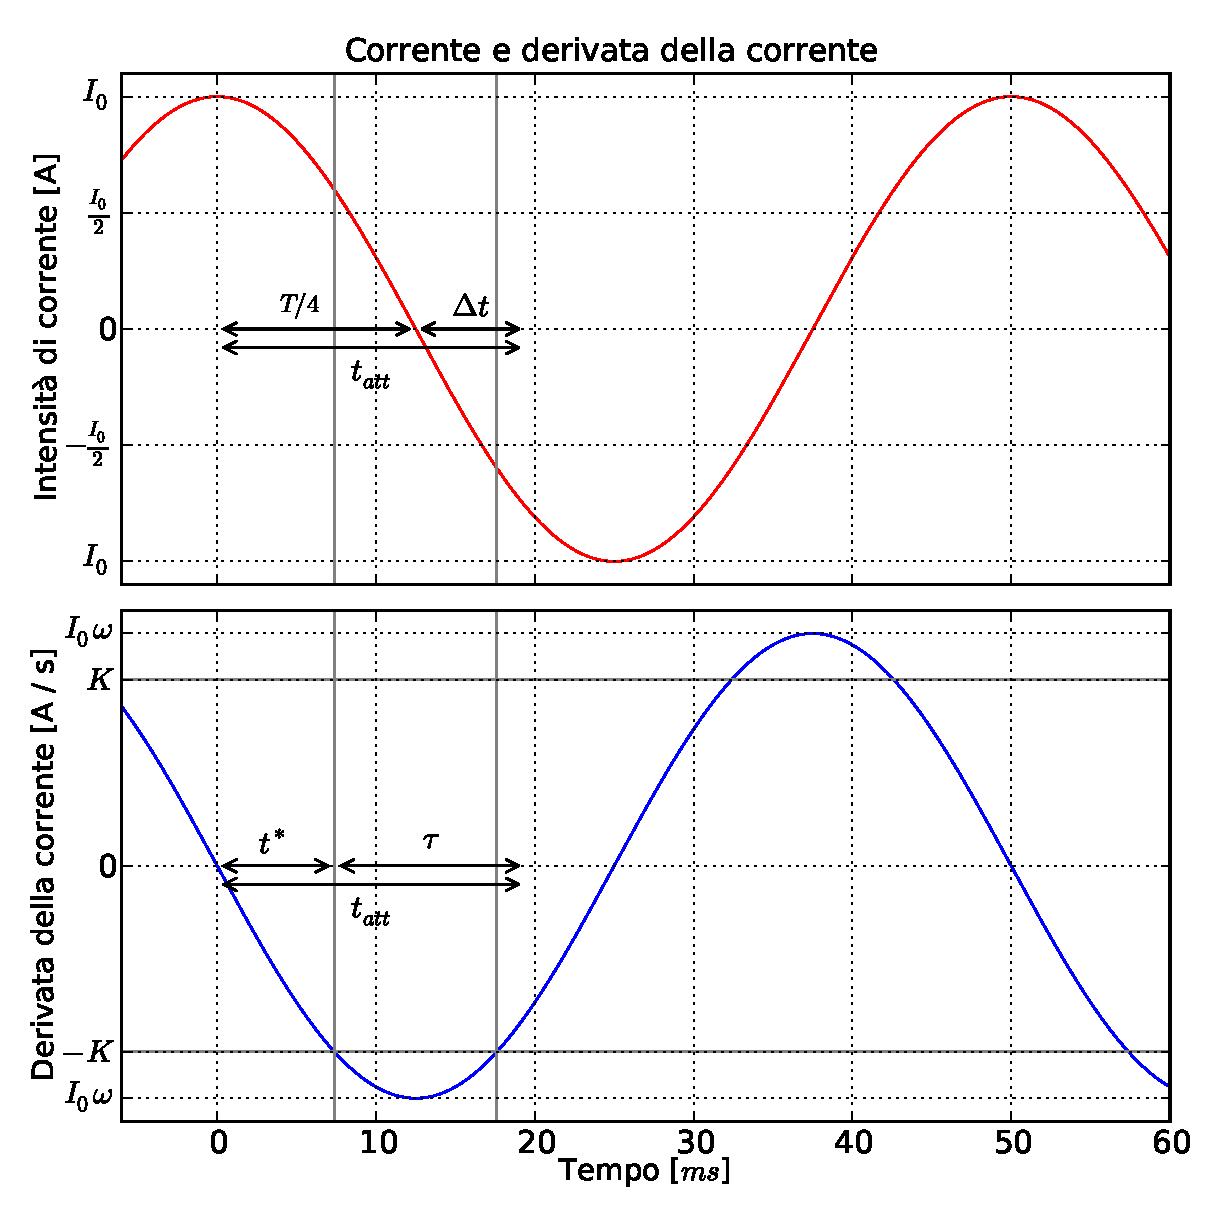
\includegraphics[height=4.2in]{gon.pdf}
    \caption{Grafico della corrente e della derivata della corrente in funzione del tempo.}
    \label{fig:gon}
\end{wrapfigure}
ricavata da considerazioni di carattere goniometrico (vedi Figura \ref{fig:gon}):\\

\noindent
\begin{minipage}{0.38\textwidth}
\begin{equation*}
t^* + \tau \,= \, t_{att} \, = \, \theta + \Delta t \, =\,\frac{T}{4} + \Delta t
\end{equation*}
\begin{equation*}
\downarrow
\end{equation*}
\begin{equation}
\tau \, = \, \frac{T}{4} + \Delta t - t^* = (10.0 \pm 0.2) ms
\label{eq:times}
\end{equation}
\end{minipage}\\

Osserviamo che sia $t^*$ che $\theta$ sono del tutto dipendenti dalla scelta della fase iniziale $\varphi$. Ciò nonostante tale dipendenza non è influente sul tempo \emph{meccanico} $\tau$. Nel caso generale le equazioni risulterebbero più complesse, ma evidenzierebbero l'indipendenza di $\tau$ dalla fase iniziale.

Inoltre il valore massimo di attivazione $t_{att}$ dovrebbe essere
\begin{equation*}
	t_{att,max} \,=\, 2 t^* + \tau = \frac{2}{\omega}arcsin\left(\frac{KR}{V_0 \omega}\right) + \tau
\end{equation*}
Osserviamo che esso dipende dalla resistenza scelta e dalla differenza di potenziale imposta al circuito.
